\section{Planteamiento del problema}
Ateniéndonos a los datos presentes en la Agenda del Agua 2030, en México, tan solo el 91.3\% de la población cuenta con servicio de agua potable y 89.9\% tiene cobertura de alcantarillado del cual, solo un 43.4\% recibe tratamiento. Las estimaciones esperadas rumbo a 2030 indican que se requerirá infraestructura para dar un tratamiento correcto a 7.157 miles de millones de metros cúbicos, generando una brecha de 4.3 miles de millones de metros cúbicos~\citep{aa2030}.\par
Tales objetivos se vuelven aún más alejados de convertirse en realidad cuando analizamos que, tan solo en Jalisco, de las 230 plantas de tratamiento a cargo del gobierno, para abril del 2024 solo 144 se encuentran en operación, con un tratamiento estimado de 16088 litros por segundo; y solamente una planta en construcción~\citep{CEAJ24}.\par
Así mismo, resulta alarmante el aumento de la temperatura y las constantes sequías, las cuales comprometen la seguridad hídrica de los gobiernos de cada país, la \cite{CNA2024} en su informe monitoreo de sequía advierte que, tan solo en México: 1899 de los 2471 municipios sufren de alguna de las 4 categorías diferentes de sequía, 366 condición anormalmente seca y tan solo 206 son los que no presentan algún tipo de afectación (ver figura \ref{fig:sequia}).
\begin{figure}[H]
	\centering
	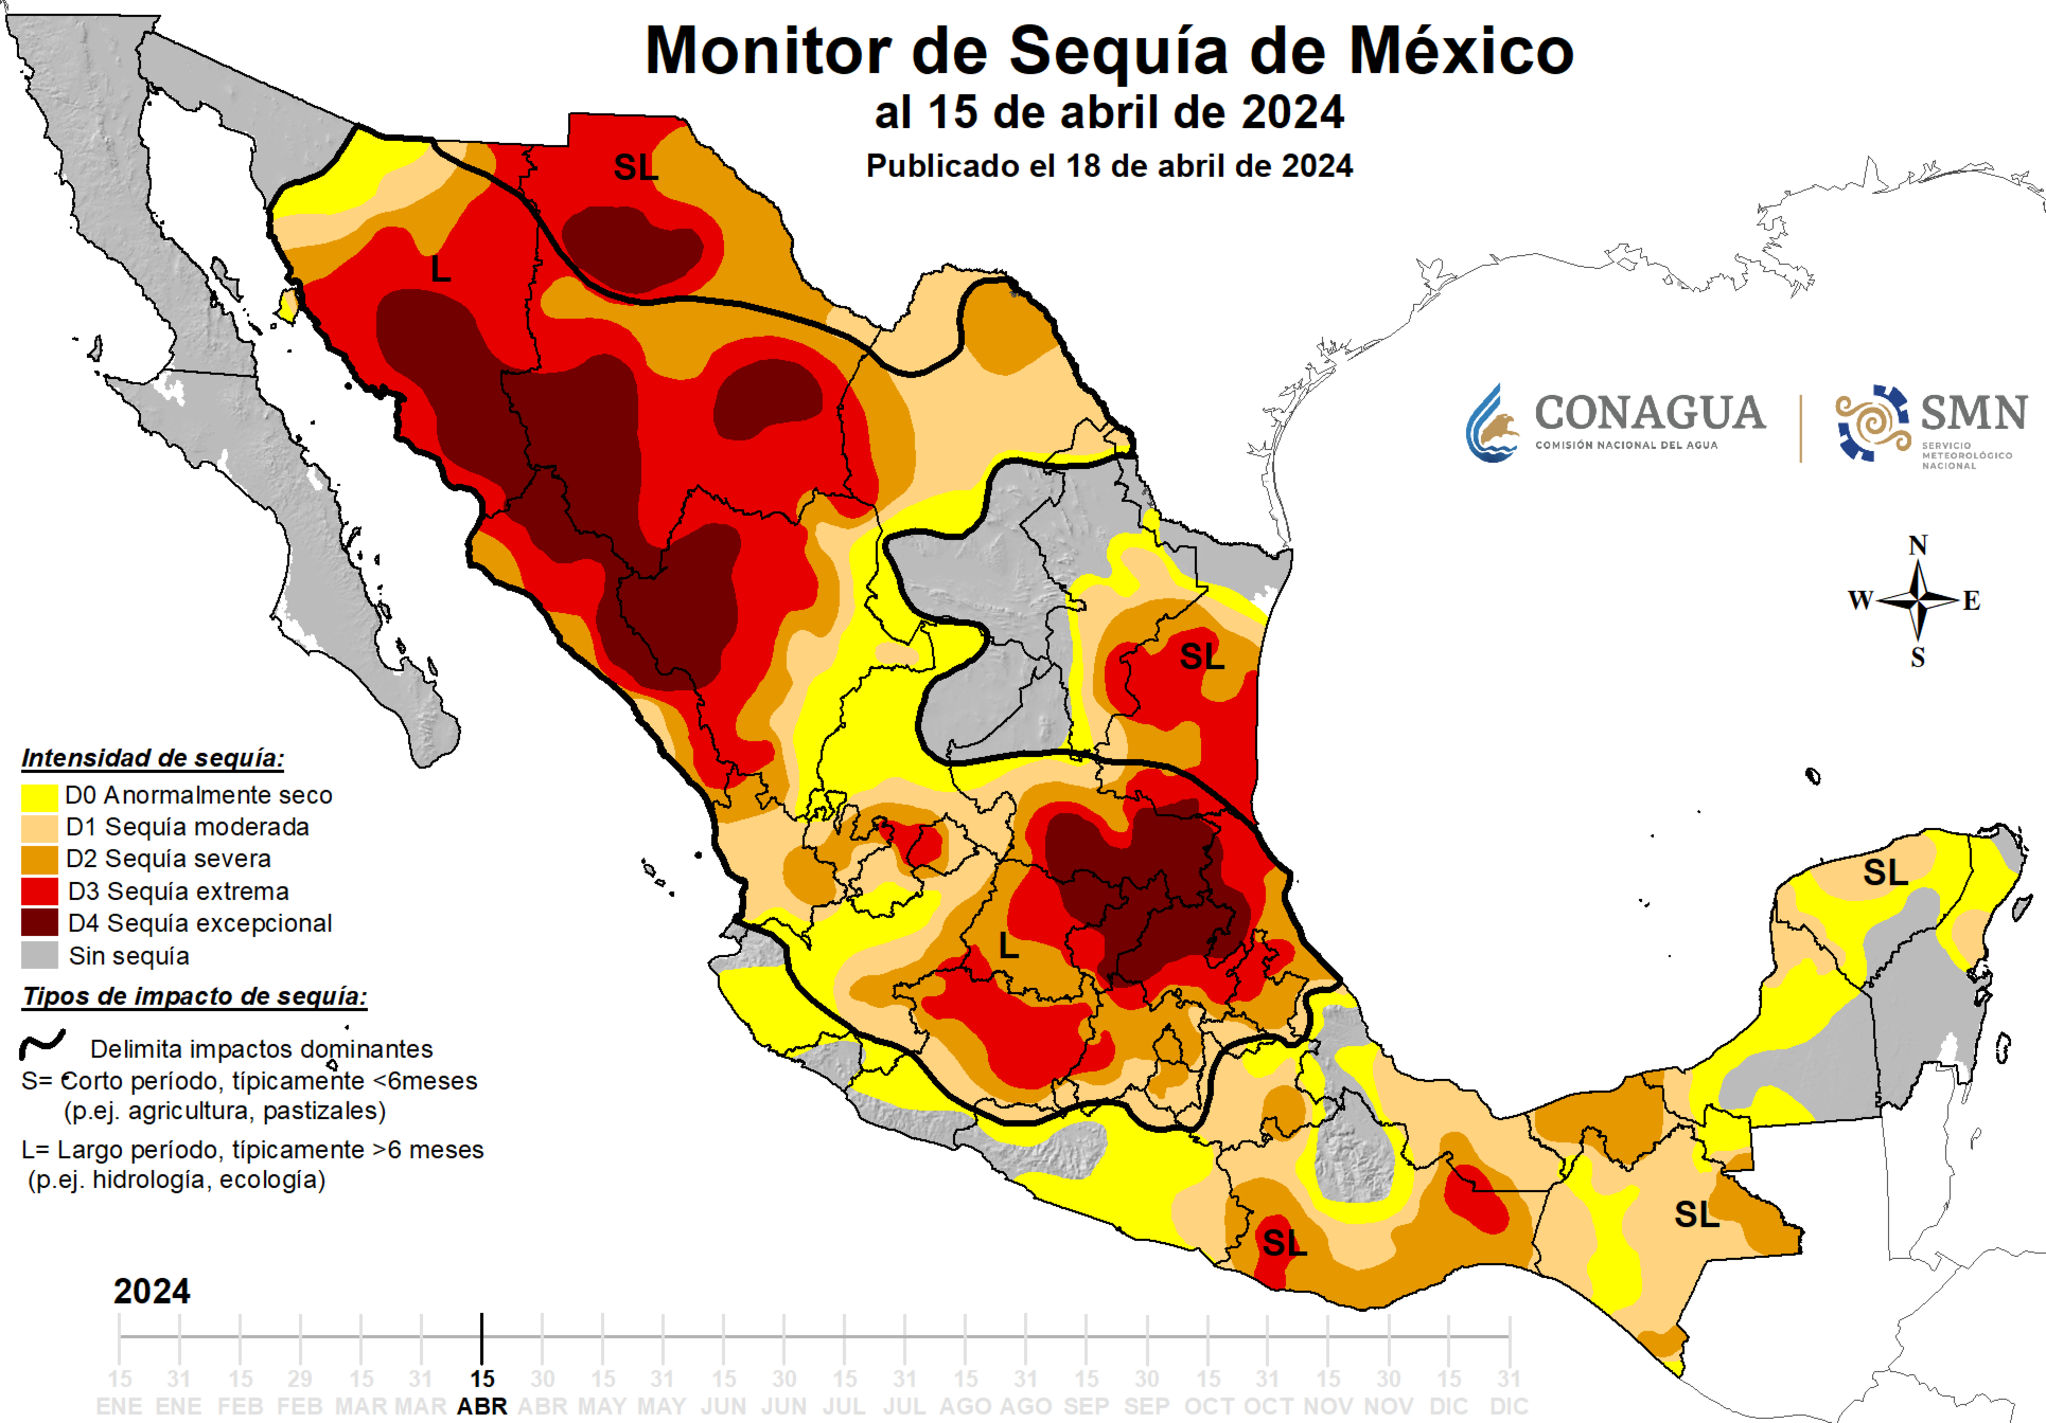
\includegraphics[scale=0.35]{../Images/Sequia.pdf}
	\\\small{Fuente: \cite{CNA2024}}
	\caption{Mapa de México dónde se muestra los niveles de sequía acorde a la intensidad al mes de abril del 2024}\label{fig:sequia}
\end{figure}
La finalidad de este proyecto es obtener las condiciones de operación que mejor se adaptan al proceso de remoción de contaminantes con el fin de estandarizar un sistema de tratamiento eficiente y de bajo coste que pueda ser utilizado en localidades que no cuenten con un proceso de tratamiento de las aguas residuales generadas por estas.